\section{設計} \label{section:design}

\subsection{データ単位でのヒュージページ割り当て}
前章で述べた通り,Apache Sparkにおいてヒュージページを使う際にはアプリケーション単位でしか
使用の有無を選択できない.これはJVMのオプションとしてJVM全体にヒュージページを使うか使わないかしか
選べないからである.

予備実験ではデータ単位での割り当てを行うための実装をSparkにおいて行った.手法としてはStorageMemoryに
あるデータを定期的にスキャンし,1ページに一定以上のサイズが含まれている場合はヒュージページに昇格するように
マークをつけていくという方式となっている.これによって一部のヒュージページ割り当てには成功したが,
一度割り当てたデータを後から昇格するため昇格に時間がかかりヒュージページの効果が現れるのが遅いことや
メモリをスキャンするためにスレッドを一時停止するためオーバーヘッドが大きいといった問題点があった.

これらを解決するために今回の提案方式ではJVMに改良を加え,データごとにヒュージページを
使うかどうか選べるようにする.この改良されたJVMを使いSparkでデータを生成する際にそのデータの
特性に合わせてヒュージページを使うかどうか選ぶことで効率的なヒュージページ割り当てを行う.
JVM側でデータの生成の際に直接ヒュージページとして生成することで昇格を待つ必要がなく,すぐに
恩恵が受けられる.また,メモリをスキャンする必要がなくなったためオーバーヘッドを気にする
必要もなくなる.

\subsection{ヒュージページ割り当てを行うデータ}
Spark では図\ref{fig:spark-memory-management}に示すような形でメモリの管理が行われている\cite{spark-memory-management}.Reserved Memory はSpark 内
部オブジェクト用に確保された領域であり固定の大きさとなっている.User Memory はユーザデー
タ構造や内部メタデータを保存する領域である.Execution Memory はSpark のタスクを実行する
ためのメモリであり,主に短命なオブジェクトのための領域である.Storage Memory はキャッシュ
したRDD などが保存される領域で主に長命なオブジェクトを保存するための領域である.Storage
Memory とExecution Memory のサイズは明確に決まっておらず,状況によって領域が移動する.

Spark アプリケーションではファイルからデータをロードし,RDD としてStorage Memory に保存,
RDD へ繰り替えし処理を行う,という構成が多いため,Storage Memory には頻繁にアクセスされる
大きなデータが保存される.そのため,ヒュージページの影響を大きく受ける領域はStorage Memory
ではないかと考えられる.
よって提案方式ではこのStorageMemoryに保存されるデータに対してヒュージページ割り当てを行う.

\begin{figure}
  \centering
  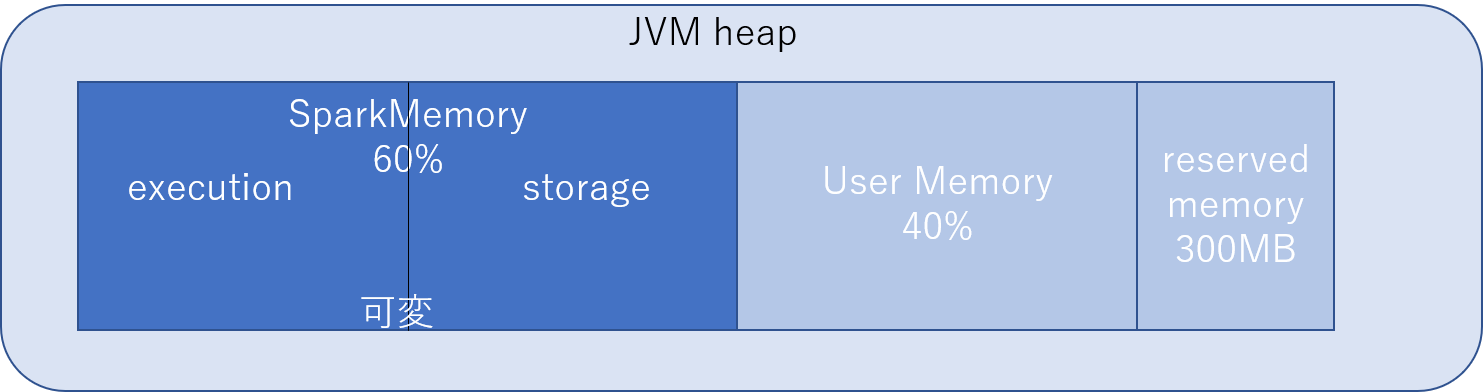
\includegraphics[scale=0.3]{figures/spark-memory-management.png}
  \caption{Sparkメモリ管理}
  \label{fig:spark-memory-management}
\end{figure}
